Las siglas GPU provienen de Graphics Processing Unit, o en español Unidad de
procesamiento gráfico. Para efectos de hardware, la GPU funciona como
coprocesador, pudiéndose utilizar de forma simultánea a la CPU y así aprovechar
el potencial que puedan ofrecer ambas al mismo tiempo.  Una GPU era un
procesador diseñado para llevar a cabo cálculos necesarios en la generación de
gráficos, sin embargo, actualmente tienen una componente multipropósito,
pudiéndose realizar distintos tipos de operaciones. Hoy en día las GPU son más
potentes y pueden incluso superar frecuencias de reloj de una CPU antigua, pero
un factor importante, es que poseen una arquitectura que permite el paralelismo
masivo.

La evolución de las tarjetas gráficas ha venido acompañado de un gran
crecimiento en el mundo de los videojuegos, las aplicaciones 3D, pero también
en cálculos y cómputos en problemas científicos, realizándose
grandes producciones de chips gráficos por parte de los fabricantes, como
NVIDIA, AMD (ex ATI). Los recientes desarrollos sobre GPU abarcan distintas
áreas de la ciencia \cite{kirk2010programming}, como problemas astrofísicos
(n-body simulation), modelamiento molecular, computación financiera, etc. En
los últimos años también han aparecido conjuntos de herramientas y compiladores
que facilitan la programación de las GPUs, como por ejemplo, NVIDIA CUDA, que
cuenta con la comunidad más activa en programación de GPUs.

\section{Arquitectura}

La arquitectura CUDA (Compute Unified Device Architecture) surgió en el año 2006, 
cuando NVIDIA lanzó sus tarjetas GeForce 8800 GTX las que por primera vez 
incluyeron elementos dirigidos específicamente a posibilitar la solución de 
problemas de propósito general. Poco después, NVIDIA lanzó el compilador CUDA 
C, el primer lenguaje de programación para desarrollar aplicaciones de propósito 
general sobre un GPU; con la finalidad de captar la mayor cantidad de 
programadores posibles que adoptasen esta arquitectura, CUDA C es un lenguaje 
muy similar a C, al cual se le agregaron un conjunto de instrucciones que harían 
posible la programación en paralelo en un sólo equipo de cómputo.

Este conjunto de instrucciones permiten que los programadores desarrollen 
aplicaciones que comunican a la CPU con la GPU para utilizar de esta última sus 
múltiples microprocesadores, sobre los cuales pueden ser ejecutadas 
simultáneamente varias tareas.

La razón de estas diferencias entre la capacidad de la CPU y la GPU, es que la
GPU está diseñada para realizar computación-intensiva, altamente paralela y por
ello está dotada de mayor cantidad de transistores que se dedican al
procesamiento de datos en las unidades aritmético-lógicas (ALU) en lugar de
almacenar datos en cache o controlar el flujo de información.

\begin{figure}[h]
    \centering
    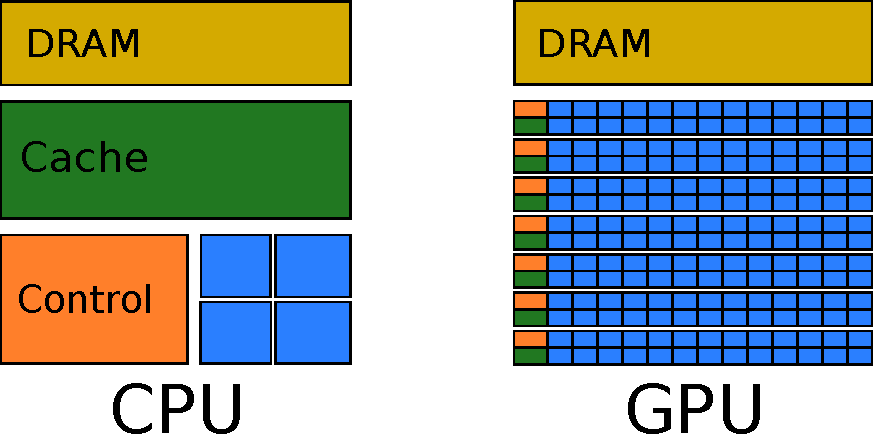
\includegraphics[width=0.8\textwidth]{images/cpu_gpu_arch.pdf}
    \caption{CPU y GPU vista general de su arquitectura}
    \label{fig:cpu_gpu_arch}
\end{figure}

Acercando más en detalle la comparación entre CPU cores y CUDA cores se puede
ver en la figura \ref{fig:cpu_gpu}.

\begin{figure}[h]
    \centering
    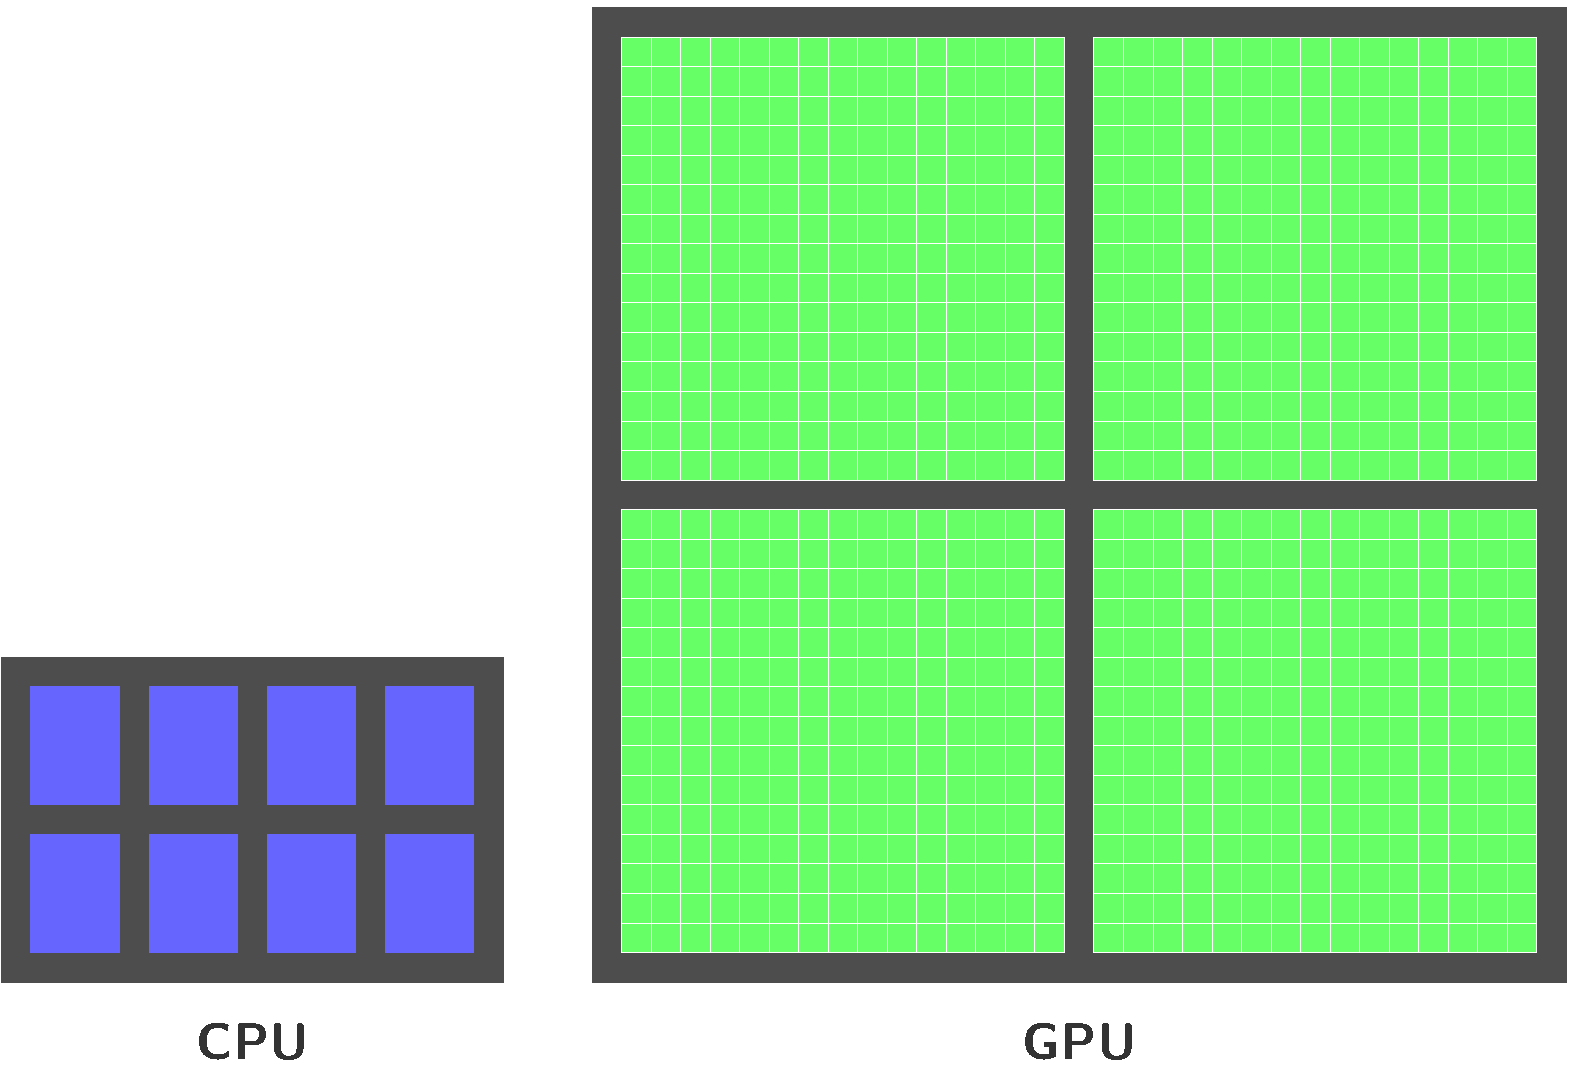
\includegraphics[width=0.5\textwidth]{images/cpu_gpu.pdf}
    \caption{CPU y GPU Layout de los núcleos}
    \label{fig:cpu_gpu}
\end{figure}

Esto implica que la GPU está especialmente diseñada para llevar a cabo gran
cantidad de operaciones en paralelo. Puesto que cada elemento de procesamiento
posee sus propias memorias locales y no se requiere habilitar un control de
flujo sofisticado. Además, la latencia por accesos a memoria se disminuye.

\newpage
\section{Lenguaje de programación CUDA}

CUDA como lenguaje de programación basado en la arquitectura presentada
anteriormente \ref{fig:cpu_gpu_arch} y está sujeta a los siguientes elementos
\ref{fig:cpu_gpu_elements}:
\begin{itemize}
 \item \textbf{Thread/Hilos}: Donde se ejecutan las funciones. Los hilos pueden
 procesarse simultáneamente y cuentan con memoria local para almacenar sus
 datos.
 \item \textbf{Blocks/Bloques}: Un conjunto de hilos que se ejecutan en un
 multiprocesador. Cada bloque cuenta con una zona de memoria, denominada
 memoria compartida, accesible para todos sus hilos.
 \item \textbf{Grid/Malla}:  Un conjunto de bloques. Cada malla se ejecuta sobre una
 GPU distinta y cuenta con memoria accesible para todos los bloques que la
 componen.
\end{itemize}

A las funciones que se ejecutan sobre la CPU se les conoce como funciones del 
HOST y las que se ejecutan sobre la GPU se denominan funciones del DEVICE.

\begin{figure}[h]
    \centering
    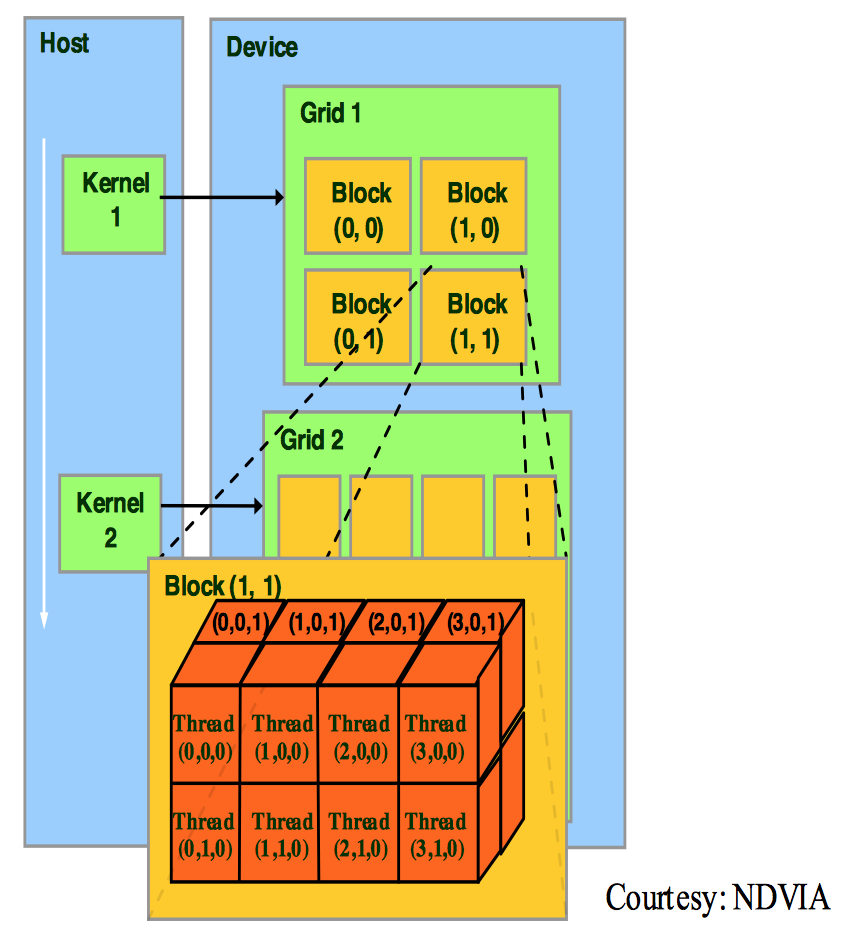
\includegraphics[height=0.5\textwidth]{images/elements.png}
    \caption{CPU y GPU elementos generales}
    \label{fig:cpu_gpu_elements}
\end{figure}

El modelo de programación de CUDA se diseñó de tal manera que tiene una curva
de aprendizaje baja para los programadores de C, que solo deberán
familiarizarse con: la forma en la que cooperan los hilos, las jerarquía de la
memoria, el uso de la memoria compartida y las instrucciones necesarias para
sincronizar las tareas que se realizan simultáneamente.

Esas pequeñas adiciones al estándar de C permiten paralelizar el problema ya
sea con una paralelización de grado fino orientada a los datos; ó una
paralización de grano grueso orientada a las tareas, también conocida como
paralelización orientada a los hilos. El reto para el programador es, decidir
de qué manera atacar el problema para dividirlo en sub-problemas que se puedan
agrupar en hilos y bloques que lo resuelvan cooperativamente y en paralelo.
Por lo tanto, debe determinarse la manera en que cooperan los hilos en el
bloque y cómo se puede escalar la solución del problema, lanzando
simultáneamente varios bloques para ser ejecutados en los núcleos que se tengan
disponibles.

